\documentclass{article}

\usepackage{amsmath}
\usepackage{amssymb}
\usepackage[english]{babel}
\usepackage{biblatex}
\usepackage{booktabs}
\usepackage[a4paper,textwidth=450pt]{geometry}
\usepackage{graphicx}
\usepackage{indentfirst}
\usepackage[utf8]{inputenc}
\usepackage{csquotes}
\usepackage{multirow}
\usepackage{physics}
\usepackage{refcheck}
\usepackage{subcaption}
\usepackage{units}
\usepackage{wrapfig}

\addbibresource{novel.bib}

\setkeys{Gin}{width=.6\textwidth}
% !TeX spellcheck = en_GB
\graphicspath{ {./images/} }

\DeclareMathOperator{\E}{\mathbb{E}}

\newtheorem{proposition}{Proposition}

\newenvironment{proof}
 {\begin{trivlist} \item[] {\bf Proof.\ }}{\hfill$\Box$ \end{trivlist}}

\title{Newsvendor Problems: A New Integrated Approach\\ to Forecasting and Optimisation}

\author{Congzheng Liu\thanks{Department of Management Science,
Lancaster University, Lancaster LA1 4YX, UK.
Email: {\tt \{c.liu19,a.n.letchford,i.svetunkov\}@lancaster.ac.uk}}
\and Adam N.\ Letchford$^*$ \and Ivan Svetunkov$^*$} % end author list

\date{Draft, 1st August 2020}

\begin{document}

\maketitle

\begin{abstract}
Newsvendor problem forms a classical and important family of stochastic optimisation problems. The standard solution approach decomposes the problem into two steps: estimation of the demand distribution, and optimisation of the production quantity (or quantities) for the given distribution. We propose a new, integrated approach, which estimates the optimal production quantity directly from the data. We prove that in the case of linear Newsvendor problem, this approach is equivalent to using quantile regression and show that it is applicable to nonlinear cases as well. Conducting experiments on simulated data we also show that the proposed approach performs at least as good as the conventional ones when applied to the classical (linear) newsvendor problem, and outperforms them, when applied to the nonlinear newsvendor problem. We also give evidence that our approach is more robust with respect to different types of model misspecification.
\\*[2mm]
{\bf Keywords:} newsvendor problems, forecasting, data-driven optimisation, sales and operations planning
\end{abstract}


%%%%%%%%%%%%%%%%%%%%%%%%%%%%%%
\section{Introduction}

Inventory control is a classical and important topic in Operations Research and Operations Management (see, e.g., the books \cite{Po02,SPP98,Zi00}). In this paper, we focus on \emph{Newsvendor Problem} (NVPs), by which we mean \emph{single-period} inventory control problem with \emph{stochastic demands}.

In early works on NVPs \cite{AHM51,MK51}, it is assumed that the demand in each time period comes from a known probability distribution. Of course, in practice, this is not the case --- a fact already noted in 1958 by Scarf \cite{Sc58}. Assuming that historical demand data is available, one can attempt to address this issue by decomposing the problem into an estimation/forecasting phase and an optimisation phase. In the first phase, one makes some assumptions (e.g., normality) regarding the underlying data generating process, and uses the past data to estimate the parameters of the model. In the second phase, one determines the order quantity (or quantities) based on the estimated parameter values. Throughout this paper, we will call this two-phase approach the \emph{disjoint} approach. An advantage of the disjoint approach is that forecasting and optimisation experts can operate independently within an organisation. This makes things easier to manage. On the other hand, as noticed by several authors \cite{BT06,BM12,Ka94,KT96,KTB20}, there are two disadvantages:
\begin{itemize}
    \item The two phases use different objective functions. Indeed, in the first phase, the objective is to minimise a function of the forecasting errors, such as the root mean square error or mean absolute error. In the second phase, however, the goal is usually to maximise expected profit.
    \item If the forecasting model is misspecified, and/or there is substantial noise in the data, then this might impact the optimisation phase in an unexpected way, probably leading to not optimal solutions. In particular, upside and downside errors may have very different effects on expected profit, due to different costs associated with over- and under-stocking.
\end{itemize}

An alternative to the disjoint approach is to use a single, \emph{integrated} approach, in which the order quantities are determined directly from the data. A simple example of an integrated approach is the \emph{quantile regression} \cite{Br16,Hu19}, which does not make assumptions about the demand distribution. Unfortunately, it can only be applied to relatively simple linear NVPs, for which one can express the optimal order quantities in terms of quantiles of demand.

In this paper, we introduce an \emph{Integrated Method for Estimation and Optimisation} (IMEO), the flexible method, which can be applied to a wide variety of NVPs, with demand processes and profit functions of different complexities. In a nutshell, the method involves forecasting the optimal order quantities instead of the demand, which is done via the maximisation of the expected profit, instead of estimating parameters via the minimisation of a function of forecast errors.

% We demonstrate that IMEO reduces to quantile regression in the case of the simplest NVP. We then perform extensive computational experiments, on several different NVPs, the results of which show that IMEO performs at least as well as the disjoint approach, according to several different measures of quality.

The rest of the paper is organised as follows. Section \ref{se:lit} provides a brief review of the relevant literature. Section \ref{se:new} presents IMEO and shows that it is a generalisation of the quantile regression. In Section \ref{se:results}, we conduct extensive simulation experiment, present and discuss the results. We then finish the paper with conclusion remarks in Section \ref{se:end}, summarising the main insights and outlining the limitations and suggesting the ares of future research.

%%%%%%%%%%%%%%%%%%%%%%%%%%%%%%
\section{Literature Review} \label{se:lit}

Since the literature on NVPs is vast, we mention here only works of direct relevance. The reader looking for more information is directed to the books on the subject \cite{Ch12,Po02,SPP98,Zi00}.

\subsection{The classical newsvendor problem} %\label{sub:lit1}

In the simplest NVP, found in textbooks \cite{Ch12}, a company purchases goods at the beginning of a time period at a cost of $v$ per unit, and aims to sell them by the end of the period at a price $p$ per unit. The demand during the period is a random variable $Y$ with known probability density function $f$ and cumulative distribution function $F$. At the end of the period, any surplus goods will lead to a \emph{holding cost} of $c_h$ per unit. On the other hand, shortage of goods during the period will lead to a \emph{shortage cost} of $c_s$ per unit. The goal is to determine an \emph{order quantity} $Q$, prior to the period, that maximises the expected profit.

For a given $Q$ and a given realisation $y$ of $Y$, the profit over the period is:
\[
    \pi(Q,y)=
    \begin{cases}
        py-vQ-c_h(Q-y),& \text{if } Q\geq y\\
        pQ-vQ-c_s(y-Q),& \text{if } Q< y.
    \end{cases}
\]
The expected value of $\pi(Q,y)$ is:
\[
    \Pi(Q) = \int_{0}^{Q} \big[ py-vQ-c_h(Q-y) \big] f(y)dy + \int_{Q}^{\infty} \big[ pQ-vQ-c_s(y-Q) \big] f(y)dy.
\]

It is common to call $c_u= p-v+c_s$ the ‘underage’ cost and $c_o = v+c_h$ the ‘overage’ cost. Some calculus then shows that the order quantity that maximises $\Pi(Q)$ is \cite{Ch12}:
\[
    Q^* = F^{-1}\left( \frac{c_u}{c_o+c_u} \right),
\]
where $F^{-1}$ is the inverse function of $F$. Thus, $Q^*$ is the $\tau$\textsuperscript{th} quantile of $f$, with $\tau=\nicefrac{c_u}{(c_o+c_u)}$. One can think of the quantity
$\tau$ as a ``target service level", since aiming for this target will bring the company maximised expected profit.

\subsection{More complex newsvendor problems} %\label{sub:lit2}

Since the introduction of NVP in the 1950s \cite{AHM51,MK51}, researchers have considered several extensions of the problem, including variants with multiple product types \cite{HW63,LL96,MS00}, quantity discounts \cite{Kh95}, different risk measures \cite{EGS95}, product substitution \cite{BAA99}, nonlinear cost functions \cite{HOS12}, non-stationary demand \cite{KWH15}, and price setting \cite{KC62,Mi59,PD99}.

For the purpose of what follows, we now explain one variant, the `Nonlinear Newsvendor Problem' (NNVP), in detail (see also \cite{BT06,HOS12,HN16,KC62,Kh95,KK18,Mi59,PSC15,PD99,Po90,Po02}). In the NNVP, the profit function takes the form:
\[
    \pi(Q,y)=
    \begin{cases}
        P(Q,y)-V(Q)-C_h(Q,y),& \text{for } Q \geq y\\
        P(Q,y)-V(Q)-C_s(Q,y),& \text{for } Q< y,
    \end{cases}
\]
where $V$, $P$, $C_h$ and $C_s$ are now \emph{functions} rather than constants.

If $\pi(Q,y)$ has a particularly simple form (e.g., if it is piecewise-linear as in classical NVP), then it may be possible to  use calculus to express the optimal order quantity as a quantile \cite{Ch12}. In general, however, a closed-form expression as a quantile is unlikely to exist \cite{HOS12,Po02}.

We now review one particular example of NNVP, taken from \cite{KK18,PD99,Ro02}, that we are going to use in our numerical experiments. The purchase cost $v$ and selling price $p$ are constants, but $C_h$ and $C_s$ are functions. Overstock items incur a constant unit penalty $\alpha > 0$, but they can be sold in a salvage market with fixed unit sales price $\beta$, with $0<\beta<v$. The demand in the salvage market is itself a random variable, with known distribution, which we denote by $u$. That is, we have:
\[
    C_h(Q,y) \, = \, \alpha[Q-y]^{+} - \beta \E \Big[ \min \big\{ [Q-y]^{+},u \big\} \Big].
\]
Moreover, the shortage penalty is proportional to the shortage quantity. That is:
\[
C_s(Q,y) =  \zeta \, \big( [y-Q]^{+} \big)^2
\]
for some constant $\zeta > 0$. This problem cannot be solved analytically, but there are known approximation methods that give adequate solutions \cite{KK18}.

\subsection{Quantile regression} \label{sub:lit3}

Returning to the classical NVP, we now consider the (more realistic) case in which the demand distribution is unknown, but we have historical demands $y_1,y_2,\dots,y_s$.
For this case, \emph{quantile regression}
has proven to perform well, and the basic idea is as follows \cite{BT06,Br16,CS19,HNS15,Hu19}:
\begin{enumerate}
\item Compute the value of $\tau$ that maximises expected profit;
\item Use quantile regression to compute an estimate of the $\tau$\textsuperscript{th} quantile of the demand in the next time period, which we denote by $\hat{y}_{s+1}^{(\tau)}$;
\item Set the order quantity $\hat{Q}_{s+1}$ to $\hat{y}_{s+1}^{(\tau)}$.
\end{enumerate}

The biggest advantage of quantile regression is that this method doesn't require the assumption of a specific demand distribution \cite{Hu19}. However, it is efficient only on large samples \cite{Hu19,RV19}. Another drawback is that the performance of this approach depends crucially on the underlying target service level. Huber \cite{Hu19} and Rudin \cite{RV19} demonstrated that the benefit of using the quantile regression method is limited to target service levels smaller than 0.8. If the target service level is higher, then much more data is needed in order to correctly estimate specific quantile.

While quantile regression can be used efficiently for the classical NVP, given enough historical data, it is not applicable for some NVPs with complex profit functions, since it becomes impossible to express the optimal order quantity as a demand quantile using calculus alone. Instead, one must resort to numerical integration and search techniques \cite{SW81}.

%\subsection{Other integrated approaches} %\label{sub:lit4}

%There exist other integrated methods. One approach is to use machine learning techniques, such as neural networks, to estimate the optimal order quantity from historical data. The application of machine learning to NVPs can be seen in \cite{CS19,OST20,RV19}. Another integrated approach is based on so-called \emph{one-shot decision theory} \cite{Guo11,GM14,Ma19}. A numerical example was shown in \cite{Guo11}, and extensions can be found in \cite{Ma19}. For the sake of brevity, we do not describe these alternative integrated methods in detail.

%%%%%%%%%%%%%%%%%%%%%%%%%%%%%
\section{Integrated Method for Estimation and Optimisation} \label{se:new}

In order to overcome the limitations of quantile regression, we propose an alternative integrated method, IMEO, based on a statistical model with a specialised loss function.

For each historical period $t\in [1,s]$, we assume that the observed demand $y_t$ is a realisation of a random variable $Y_t$. Then, in principle, there exists an order quantity, say $Q_t^*$, that maximises the expected profit given $Y_t$ and the function $\Pi$. Thus, if we had set $Q_t$ to $Q_t^*$ prior to observing the true demand $y_t$, we would have maximised our expected profit in period $t$. Putting it another way, if we could somehow uncover the structure of the unobservable time series of orders $\big\{ Q_1^*,\dots,Q_s^* \big\}$, we would be able to estimate $Q_{s+1}^*$ directly.

Of course, in practice, the distribution of $Y_t$ is unknown, and the values $Q_t^*$ are not observable. So we approximate the $Q_t^*$ values using a linear regression model. For each $t$, the regression model yields an estimate of $Q^*_t$, which we denote by $\hat{Q}_t$. The estimate $\hat{Q}_{s+1}$ can then be used as the order quantity in the next time period.

The crucial feature of IMEO is that, instead of using the standard loss functions (such as least squares or maximum likelihood) to estimates the regression parameters, we find the parameters that maximise the empirical expected profit function $\sum_{t=1}^s{\pi \big( \hat{Q}_t,y_t \big)}$. This can be expressed as:
\[
    \hat{\boldsymbol{\beta}}=\text{argmax}_{\boldsymbol{\beta}\in \mathbb{R}^{p+1}}\displaystyle\sum_{t=1}^s{\pi(\hat{Q}_t,y_t)},
\]
assuming that the orders can be represented in a form of some sort of function of a set of explanatory variables:
\[
    \mathbf{\hat{Q}}=g\left(\mathbf{X},\boldsymbol{\beta}\right).
\]
In the special case, this can be modelled using the linear regression, expressed as:
\[
    \mathbf{\hat{Q}}=\mathbf{X}\boldsymbol{\beta},
\]
where
\[
    \mathbf{\hat{Q}}=
    \begin{pmatrix}
        \hat{Q}_1\\
        \hat{Q}_2\\
        \vdots\\
        \hat{Q}_s
    \end{pmatrix}, \quad
    \mathbf{X}=
    \begin{pmatrix}
        \mathbf{x}_1^{\mathsf{T}}\\
        \mathbf{x}_2^{\mathsf{T}}\\
        \vdots\\
        \mathbf{x}_s^{\mathsf{T}}
    \end{pmatrix}=
    \begin{pmatrix}
        1&x_{11}&\cdots &x_{1p}\\
        1&x_{21}&\cdots &x_{2p}\\
        \vdots &\vdots &\ddots &\vdots \\
        1&x_{s1}&\cdots &x_{sp}
    \end{pmatrix}, \quad
    \boldsymbol{\beta}=
    \begin{pmatrix}
        \beta_0\\
        \beta_1\\
        \beta_2\\
        \vdots\\
        \beta_{p}
    \end{pmatrix}.
\]
Here, $\mathbf{x}_t^{\mathsf{T}}$ is the $t$-th row of the matrix of explanatory variables $\mathbf{X}$, and $p$ is the number of variables. We remark that, while we present the linear regression model here, dynamic models, such as ARIMA \cite{Box76} or ETS \cite{Hy08}, could be used instead just as efficiently.

After estimating the model, we can set our next order quantity to $\hat{Q}_{s+1}$, given the values of explanatory variables.

It can be shown that in the case of the classical NVP, the proposed method has the following statistical properties:
\begin{proposition}[Scale and shift invariance]
For any $a>0$, $\gamma\in \mathbb{R}^{p+1}$, we have
\[
    \hat{\boldsymbol{\beta}}(a\mathbf{y},\mathbf{X})=a\hat{\boldsymbol{\beta}}(\mathbf{y},\mathbf{X}).
\]
\[
    \hat{\boldsymbol{\beta}}(\mathbf{y}+\mathbf{X}\gamma,\mathbf{X})=
    \hat{\boldsymbol{\beta}}(\mathbf{y},\mathbf{X})+\gamma.
\]
\end{proposition}
\begin{proof}
See Appendix \ref{app:A}.
\end{proof}

\begin{proposition}[Invariance under reparameterization]
Given any $(p+1)\times (p+1)$ non-singular matrix $A$, we have
\[
        \hat{\boldsymbol{\beta}}(\mathbf{y},\mathbf{X}A)=A^{-1}\hat{\boldsymbol{\beta}}(\mathbf{y},\mathbf{X}).
\]
\end{proposition}
\begin{proof}
See Appendix \ref{app:B}.
\end{proof}

Another interesting feature of IMEO is that it reduces to quantile regression in the case of the classical NVP (see Appendix \ref{app:C}). Therefore, again in the classical case, our method inherits the desirable properties of quantile regression, such as consistency \cite{Koe05}, efficiency \cite{KM99} and asymptotic normality \cite{KHM05} of the estimates of parameters.

%%%%%%%%%%%%%%%%%%%%%%%%%%%%%%
\section{Computational Experiments} \label{se:results}

In order to assess the performance of IMEO and to understand its strengths and weakness, we conduct a simulation experiment. We start the discussion with subsection \ref{sub:exp1}, where the simplest case is studied, in which the profit function is linear and the underlying data generation process (DGP) is known. Then the case in which the profit function is nonlinear is discussed in Subsection \ref{sub:exp2}. Finally, we discuss more complicated scenarios with the misspecified models with both linear and non-linear NVPs in respective Subsections \ref{sub:exp3} and \ref{sub:exp4}.


%%%%%%%%%% Experimental setup %%%%%%%%%%
\subsection{Experimental setup}

In our experiments, we consider NVPs with quarterly demand data, and we generate data from a seasonal ARIMA$(1,0,0)(1,0,0)_4$ process with $\theta=0.3$, $\Theta=0.5$, and constant level $500$. We also assume that the error term of the DGP follows a normal distribution $\mathcal{N}(0,200^2)$. We chose seasonal ARIMA model as one of the popular statistical models, often used for experiments in research (for example, see the review paper on supply chain forecasting \cite{SBBKN16}). We experimented with other models for the DGP, and the results were very similar to the ones presented below.

For each of the cases, we simulated 20,000 sets of demand data, each consisting of 4800 observations. From each set, we extract sequences of lengths 40, 120, 480 and 1200. These were then used in order to explore how the amount of available data affects the performance of each method. For each set of demand data and each method, we computed $\hat{Q}_{s+1}$, the 1-step ahead forecast of orders. We then computed the following three quantities:
\begin{enumerate}
    \item Percentage Profit Loss:  $PPL=\frac{\pi(y_{s+1},y_{s+1})-\pi(\hat{Q}_{s+1},y_{s+1})}{\pi(y_{s+1},y_{s+1})}$, which shows the percentage of profit that will be lost due to using each method instead of knowing the true demand. In the ideal situation this should be equal to zero.
    \item Service Level: $SL=\frac{\mathbb {I}{(\hat{Q}_{s+1}>y_{s+1})}}{20,000}$, where $\mathbb {I}(\cdot)$ is the indicator function, equal to 1 if the condition inside it is satisfied. This measure shows the achieved service level. In the ideal situation this should correspond to the target service level.
    \item Fill Rate: $FR=\frac{\min\{\hat{Q}_{s+1},y_{s+1}\}}{y_{s+1}}$, which shows how the demand is serviced. In the ideal situation it should be equal to one.
\end{enumerate}

In our proposed method (``IMEO"), we use limited-memory BFGS \cite{LN89} as the optimisation algorithm for the estimation of $\hat{\boldsymbol{\beta}}$. Besides the proposed method, three benchmark methods are also considered:
\begin{itemize}
    \item A disjoint method (``DJ"), that estimates the parameters of the model in the first phase, and determines the optimal order quantity in the second phase.
    \item An integrated method that uses Quantile Regression (``QR") in order to determine the order quantity.
    \item Finally, we use DJ with the exact model and parameters from the DGP to perform a forecast, and determine the order quantity accordingly. This last method is ``idealised", since, in real life, one would not know the true model or true parameters of demand. We call this last method ``DGP".
\end{itemize}


%%%%%%%%%% Correct model %%%%%%%%%%
\subsection{When the true model is known}
In this scenario, we assume that the true model ARIMA$(1,0,0)(1,0,0)_4$ with constant is known, but its parameters need to be estimated. In all the methods, it is also assumed that the error term follows normal distribution with unknown variance.

%%%%%%%%%% Correct: Linear case %%%%%%%%%%
\subsubsection{Linear case} \label{sub:exp1}

We conduct several experiments with combination of costs that give service levels of 0.3, 0.5 and 0.63. Other levels can also be considered, but in additional experiments that we have conducted, we have not found any significant changes in performance of the approaches.

Initially, we choose the following parameters for our (linear) profit function:
\begin{itemize}
    \item $p=20$, $v=10$, $c_h=-3$, $c_s=-7$.
\end{itemize}
One can check that the corresponding pair $\big( c_u,c_o \big)$ is $(3,7)$, and the target service level evaluates to $0.3$.

\begin{figure}[htb]
\centering
\caption{Percentage profit loss vs. data size at 0.3 target service level}
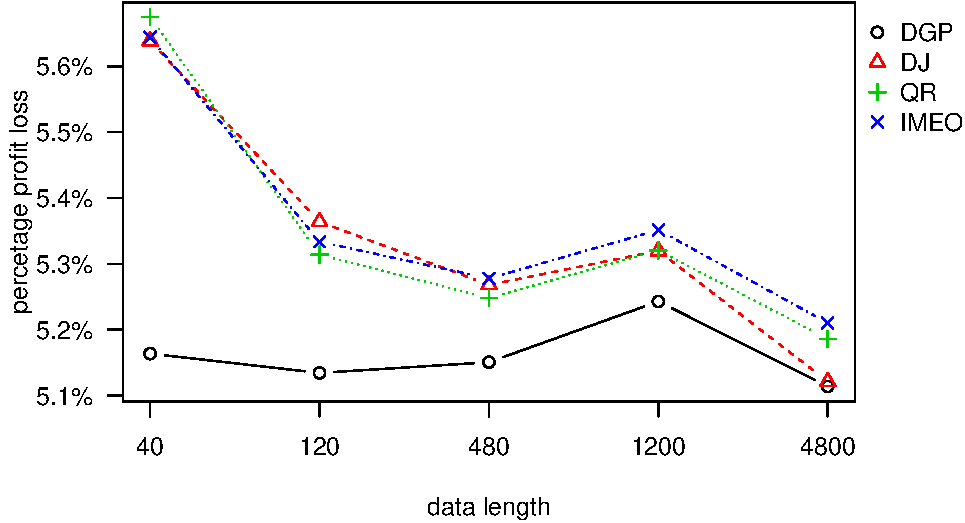
\includegraphics{ppl0.3.pdf}
\label{fig:ppl0.3}
\end{figure}

Figure \ref{fig:ppl0.3} shows the average percentage profit loss obtained when the target service level was set to $0.3$. As one would hope, the losses for all methods converge as the sample size increases. It is also apparent that IMEO and QR have very similar performance. This is to be expected, given that IMEO is equivalent to QR in the linear NVP case. Another thing to note is that the integrated approaches perform very similar to the disjoint one, which is also expected, given the knowledge of the true model and the simplicity of the NVP.

\begin{figure}[htb]
\centering
\caption{Service level vs. sample size at 0.3 target service level}
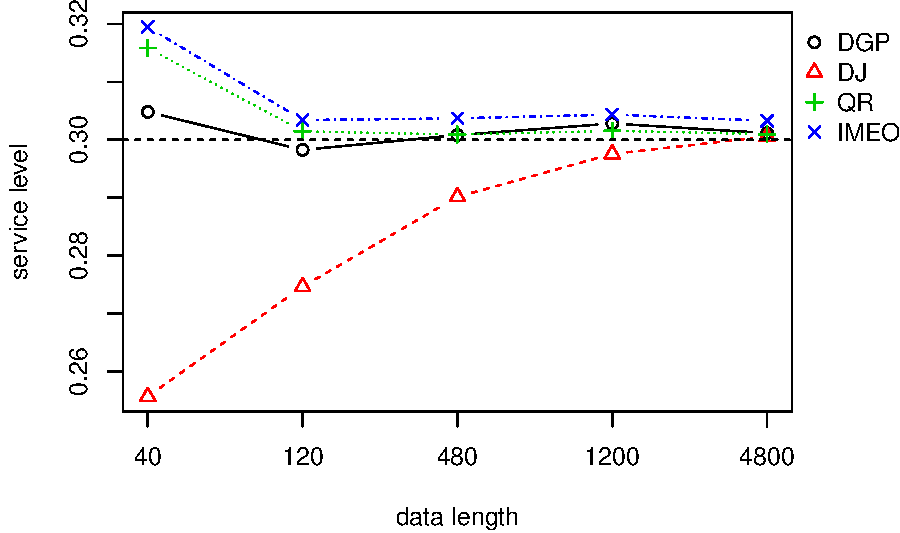
\includegraphics{sl0.3.pdf}
\label{fig:sl0.3}
\end{figure}

Figure \ref{fig:sl0.3} represents the average service level, i.e., the proportion of iterations in which the demand was satisfied in the simulation. We see that all four methods converge to the desired target of 0.3 as the sample size grows. Interestingly, DJ approaches the target from below, while IMEO and QR approach slightly over estimate the level on small samples. A possible explanation of this phenomenon is that in the first phase of DJ, the estimated variance tends to be larger than the true variance when the sample size is small. This causes the estimated order quantities to be further from the mean than they should be, and leads to lower than needed SL. On the other hand, the integrated methods take the underage and overage costs into account. For the given cost parameters, over-stocking is less costly than under-stocking, which leads to a higher service level than needed.

\begin{figure}[ht]
\centering
\caption{Fill rate vs. sample size at 0.3 target service level}
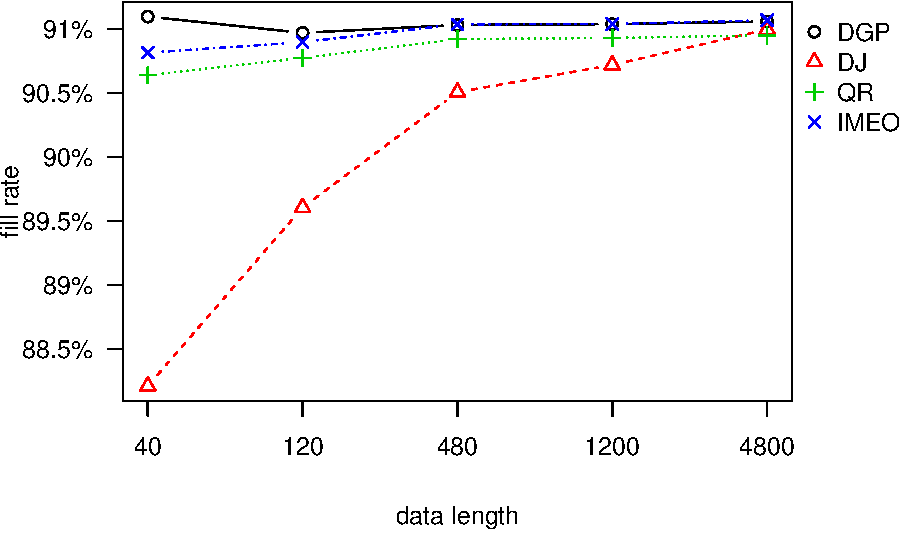
\includegraphics{fr0.3.pdf}
\label{fig:fr0.3}
\end{figure}

Figure \ref{fig:fr0.3} represents the average fill rate. As one might expect, the performance of all methods improves with the growth of the sample size. The thing to note is that the DJ requires a much larger sample size than other integrated methods in order to achieve the same FR, although the differences between the DJ and other methods are not very big (only a couple of percent points). The possible explanation of this behaviour of DJ is probably similar to the situation with the service levels.

Next, we explore whether the target service level has a significant effect on the performance of the methods. Specifically, we considered the following two alternative parameter settings:
\begin{itemize}
    \item $p=20$, $v=8$, $c_h=-3$, $c_s=-7$
    \item $p=20$, $v=8$, $c_h=3$, $c_s=7$.
\end{itemize}
These correspond to pairs $\big( c_u,c_o \big)$ are $(5,5)$ and $(19,11)$, respectively, leading to the target service levels of $0.5$ and $0.63$, respectively.

The relevant data is given in Tables \ref{tab:level_effect40} and \ref{tab:level_effect4800}, for the cases of sample sizes $s=40$
and $s=4800$, respectively. The best cases (excluding DGP, which is expected to be the best by construct) are marked in boldface for each of the error measures and each of service levels.

\begin{table}[htb]
\caption{Target service level effect with $s=40$}
\label{tab:level_effect40}
\centering
\resizebox{\linewidth}{!}{
\begin{tabular}{ccccccccccccc}
\toprule
\multicolumn{1}{c}{\textbf{ }} & \multicolumn{4}{c}{\textbf{Percentage profit loss}} & \multicolumn{4}{c}{\textbf{Service level}} & \multicolumn{4}{c}{\textbf{Fill rate}} \\
\cmidrule(l{3pt}r{3pt}){2-5} \cmidrule(l{3pt}r{3pt}){6-9} \cmidrule(l{3pt}r{3pt}){10-13}
Target service level & DGP & DJ & QR & IMEO & DGP & DJ & QR & IMEO & DGP & DJ & QR & IMEO\\
\midrule
0.5 & 4.9\% & 5.3\% & 5.3\% & \textbf{5.2\%} & 0.50 & 0.44 & \textbf{0.50} & \textbf{0.50} & 95.2\% & 93.4\% & 94.7\% & \textbf{94.8\%}\\
0.63 & 13.8\% & 15.1\% & 15.0\% & \textbf{14.8\%} & 0.63 & 0.58 & \textbf{0.62} & \textbf{0.62} & 97.1\% & 95.8\% & \textbf{96.6\%} & \textbf{96.6\%}\\
0.3 & 5.2\% & \textbf{5.6\%} & 5.7\% & \textbf{5.6\%} & 0.30 & 0.26 & \textbf{0.32} & \textbf{0.32} & 91.1\% & 88.2\% & 90.6\% & \textbf{90.8\%}\\
\bottomrule
\end{tabular}}
\end{table}

We can see from Table \ref{tab:level_effect40} that IMEO performs consistently better than the other approaches on the small sample, regardless of the target service level, although the difference in performance between the methods is not substantial. QR is the second best approach in this scenario.

\begin{table}[htb]
\caption{Target service level effect with $s=4800$}
\label{tab:level_effect4800}
\centering
\resizebox{\linewidth}{!}{
\begin{tabular}{ccccccccccccc}
\toprule
\multicolumn{1}{c}{\textbf{ }} & \multicolumn{4}{c}{\textbf{Percentage profit loss}} & \multicolumn{4}{c}{\textbf{Service level}} & \multicolumn{4}{c}{\textbf{Fill rate}} \\
\cmidrule(l{3pt}r{3pt}){2-5} \cmidrule(l{3pt}r{3pt}){6-9} \cmidrule(l{3pt}r{3pt}){10-13}
Target service level & DGP & DJ & QR & IMEO & DGP & DJ & QR & IMEO & DGP & DJ & QR & IMEO\\
\midrule
0.5 & 4.9\% & \textbf{4.9\%} & 5.0\% & 5.0\% & 0.50 & 0.50 & 0.50 & 0.50 & 95.3\% & \textbf{95.2\%} & \textbf{95.2\%} & \textbf{95.2\%}\\
0.63 & 13.8\% & \textbf{13.8\%} & 14.0\% & 14.0\% & 0.63 & 0.63 & 0.63 & 0.63 & 97.0\% & \textbf{97.0\%} & \textbf{97.0\%} & 96.9\%\\
0.3 & 5.1\% & \textbf{5.1\%} & 5.2\% & 5.2\% & 0.30 & 0.30 & 0.30 & 0.30 & 91.1\% & 91.0\% & 91.0\% & \textbf{91.1\%}\\
\bottomrule
\end{tabular}}
\end{table}

When it comes to large samples (Table \ref{tab:level_effect4800}), IMEO and QR perform slightly worse than DJ, although the difference between the methods is not substantial as well. This holds for all target service levels irrespective of the error measures. A thing to note is that the PPL is particularly high for all the methods when the target service level is 0.63. This is probably due to the relatively large overage and underage costs in that case.

Summarising, we can see that IMEO does at least as good as the classical disjoint method and quantile regression in different scenarios, in the linear NVP, when the model is correctly specified.


%%%%%%%%%% Correct: Nonlinear case %%%%%%%%%%
\subsubsection{Nonlinear profit function} \label{sub:exp2}

In this subsection, we examine the relative performance of the methods when applied to the NNVP. As before, we assume that the true model for the demands is known. We use the following nonlinear profit function \cite{KK18}:
\[
    \pi(Q,y)=
    \begin{cases}
        20y-8Q-4(Q-y)+5\E[\min \{(Q-y),u\}],& \text{if } Q\geq y\\
        20Q-8Q-0.01(y-Q)^2,& \text{if } Q< y,
    \end{cases}
\]
where $u\sim \mathcal{N}(30,5^2)$. Given that the target service level does not have a closed form in the NNVP, one can use the technique mentioned in \cite{KK18}, or other numerical approaches, to verify that it is approximately equal to 0.56.

Since the nonlinearity makes it impossible to apply QR (as discussed in Subsection \ref{sub:lit3}), we present results only for DJ and IMEO, together with the ``idealised" method based on the DGP. Moreover, we found that the FR plots were simiilar in all scenarios and do not give any additional important information, therefore, we do not present them in what follows.

Figure \ref{fig:non} shows the PPL and SL of each method, for each sample size. It is apparent that both DJ and IMEO methods perform well in terms of PPL, with very similar values for all sample sizes. IMEO is slightly better on small samples (similar to Subsection \ref{sub:exp1}), but the differences in performance between the methods are not substantial. When it comes to SL, the picture is similar to what we have observed in Subsection \ref{sub:exp1}: the SL of IMEO is very close to the the target service level even when the sample size is small, while the disjoint method needs more data to reach the target service level, and it approaches it from below. The reason for such performance is similar to the one discussed in Subsection \ref{sub:exp1}. As expected, both methods converge to the DGP values in both PPL and SL with the increase of the sample size, the methods.

\begin{figure}[ht]
\centering
\caption{Performance vs. sample size with nonlinear profit function}
\begin{subfigure}[b]{0.48\textwidth}
\centering
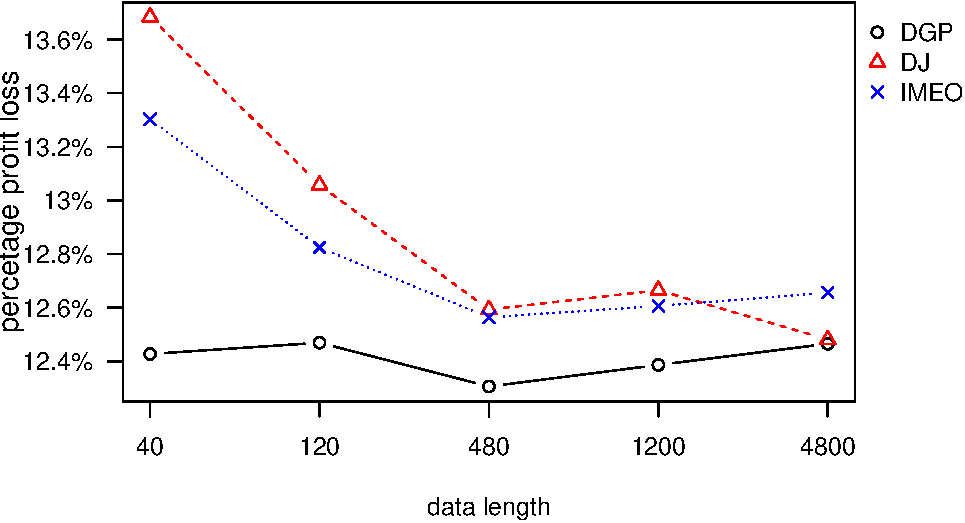
\includegraphics[width=\textwidth]{nonlinearppl.pdf}
\caption{percentage profit loss vs. data size}
\end{subfigure}
\hfill
\begin{subfigure}[b]{0.48\textwidth}
\centering
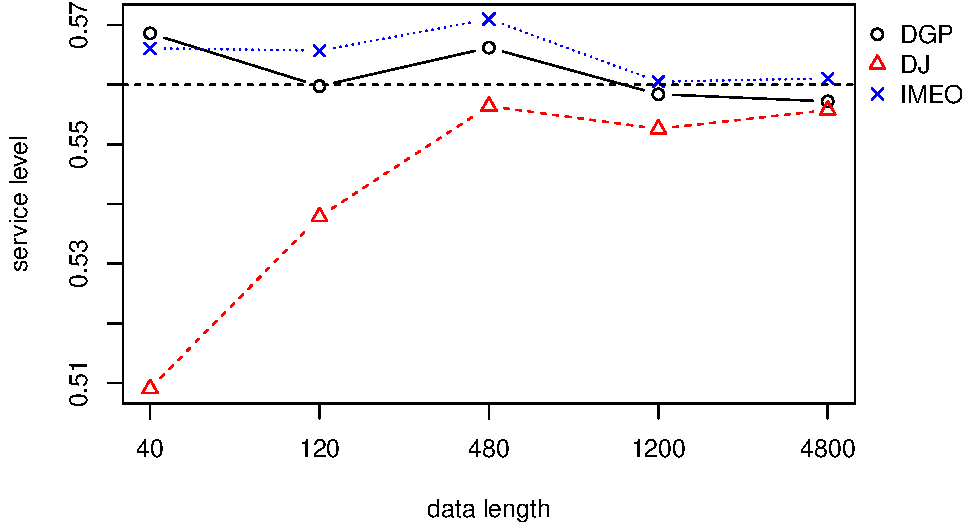
\includegraphics[width=\textwidth]{nonlinearsl.pdf}
\caption{service level vs. data size}
\end{subfigure}
\label{fig:non}
\end{figure}

We would like to stress that, unlike disjoint method, IMEO does not need any complicated numerical optimisation or simulation methods to estimate the optimal order quantity -- it does that directly. In addition, we have found that in our experiments it typically required less computational time than the disjoint method: approximately only $\nicefrac{1}{10}$ amount of time spend on DJ is needed for IMEO, when $s=40$. Besides, the IMEO results presented above are generated by limited-memory BFGS, which cannot guarantee a global optimum. One can apply other algorithms so as to balance between profit achieved and computational time.

Overall, we see that IMEO performs at least as good as DJ in the scenario, when the true model is known. Now we move to more realistic case of model misspecification.


%%%%%%%%%% Wrong model %%%%%%%%%%
\subsection{When the true model is not known}

Next, we examine the effect of \emph{model misspecification} on the relative performance of the various methods. We consider three scenarios:
\begin{enumerate}
    \item Model omits important variable, which typically leads to biased estimates of parameters;
    \item Model has redundant variables, which usually leads to ineficient estimates of parameters;
    \item The assumed distribution of error term is wrong.
\end{enumerate}
While in reality there can be other scenarios, the proposed three cover the main possible issues with the model misspecification.

We don't include QR method in further discussions because in the linear case it performs similar to IMEO, while in the nonlinear one it cannot be used.


%%%%%%%%%% Wrong: Linear case %%%%%%%%%%
\subsubsection{Linear case} \label{sub:exp3}

We first consider the situation in which applied models omit important variables (i.e., under-parameterised): the seasonal order of ARIMA is dropped in the estimation and the solution of the NVP. In other words, when estimating the optimal order quantity, we apply AR$(1)$ model with constant.

\begin{figure}[ht]
\centering
\caption{Performance vs. sample size with under-parameterised linear model}
\begin{subfigure}[b]{0.48\textwidth}
\centering
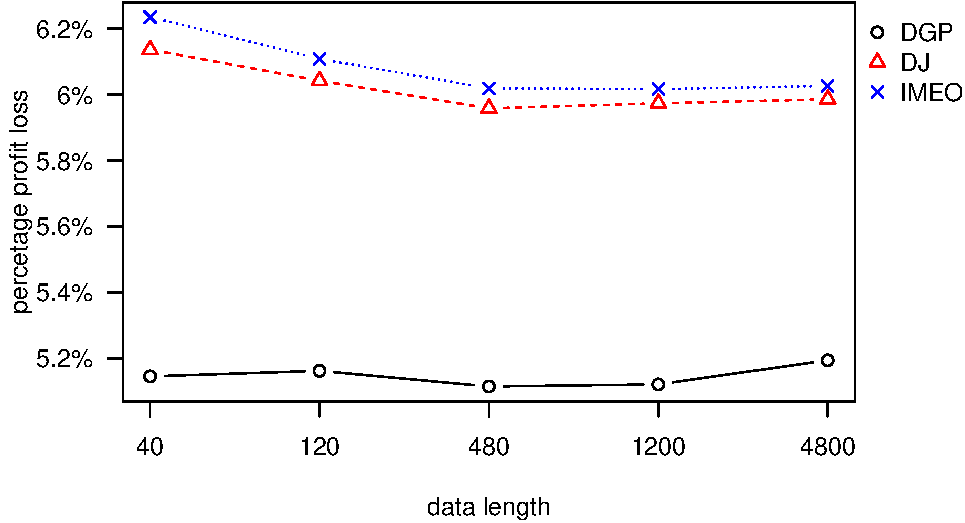
\includegraphics[width=\textwidth]{AR(1)ppl.pdf}
\caption{percentage profit loss vs. data size}
\end{subfigure}
\hfill
\begin{subfigure}[b]{0.48\textwidth}
\centering
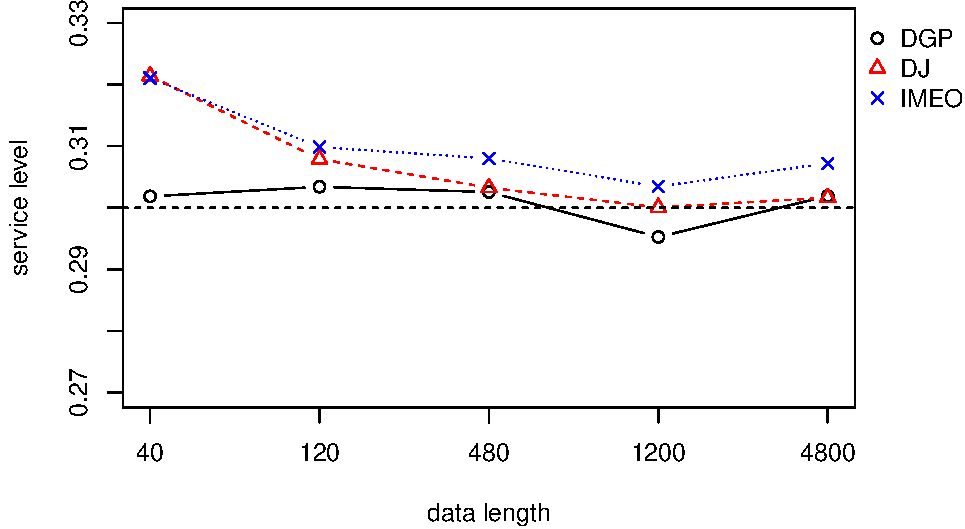
\includegraphics[width=\textwidth]{AR(1)sl.pdf}
\caption{service level vs. data size}
\end{subfigure}
\label{fig:mis_under}
\end{figure}

The PPL and SL for this case are shown in Figure \ref{fig:mis_under}. By comparing with Figure \ref{fig:ppl0.3}, we see that the use of an under-parameterised model causes both DJ and IMEO to incur small additional losses in PPL, irrespective of the sample size. This is expected, as the seasonal pattern in the data is ignored by the models. These losses do not significantly improve as the number of data points increases, because seasonality plays a key role when making one-step ahead forecasts. When it comes to the service level, both approaches perform similar, reaching the target on larger samples. But when it comes to small samples, they both reach higher than needed levels. Interestingly, the performance of DJ and IMEO is similar, even though they are very different approaches.% This could be because the assumptions about the distribution of error term are correct.

We also consider the situation in which the applied model contains redundant variables (i.e., over-parameterised). Specifically, we apply ARIMA$(2,0,0)(1,0,0)_4$ model to the data.

\begin{figure}[ht]
\centering
\caption{Performance vs. sample size with over-paramaterised linear model}
\begin{subfigure}[b]{0.48\textwidth}
\centering
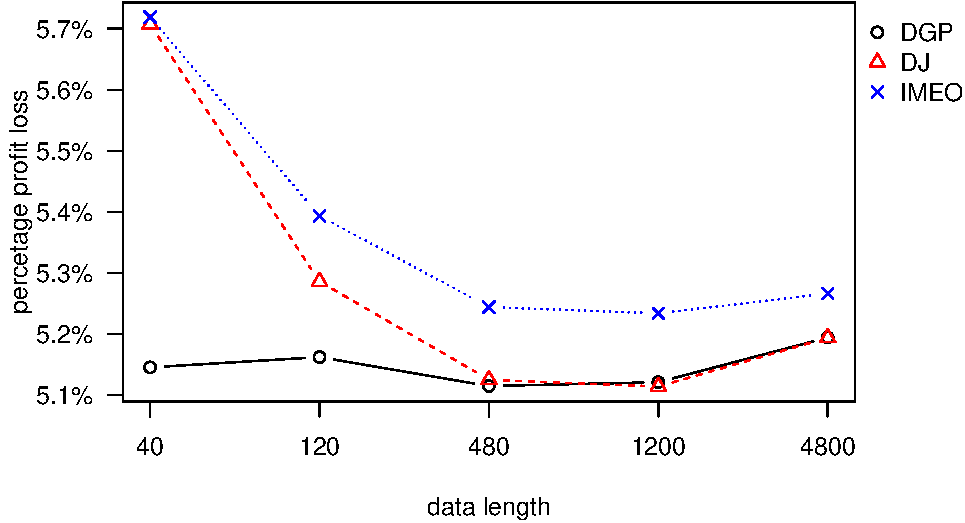
\includegraphics[width=\textwidth]{SAR(2)(1)_4ppl.pdf}
\caption{percentage profit loss vs. data size}
\end{subfigure}
\hfill
\begin{subfigure}[b]{0.48\textwidth}
\centering
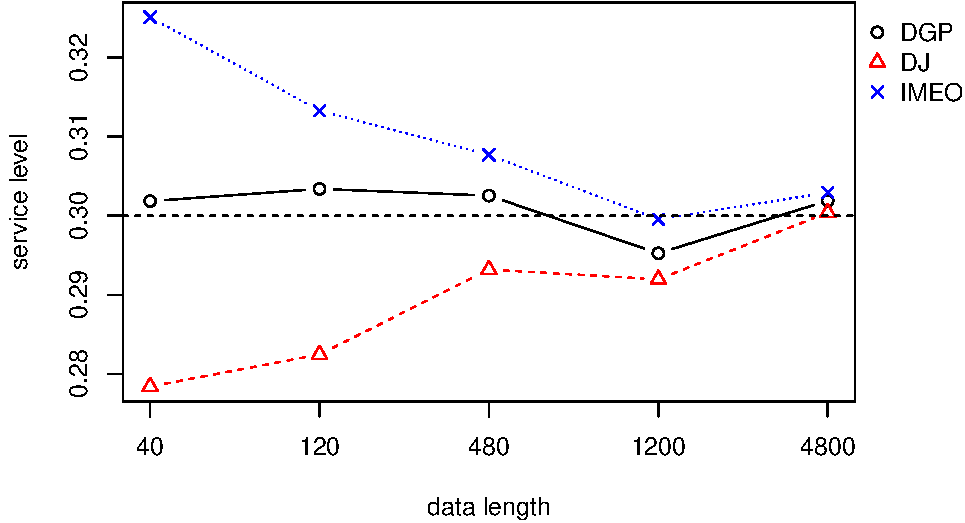
\includegraphics[width=\textwidth]{SAR(2)(1)_4sl.pdf}
\caption{service level vs. data size}
\end{subfigure}
\label{fig:mis_over}
\end{figure}

The PPL and SL for this case can be seen in Figure \ref{fig:mis_over}. Both DJ and IMEO incur a loss in profit, as before. Now, however, the profit loss decreases with the increase of the sample size. This can be explained by a well-known statistical phenomenon of estimating models with redundant variables \cite{FG67}: they tend to lead to less efficient estimates of parameters on small samples but do not lead to systematic bias (as omitted variables typically do). As for the service level, it can be seen that both methods asymptotically converge to the target, but tend to be less precise on small samples with IMEO reaching higher level than needed and DJ leading to the lower values. In terms of SL, the methods perform similar to the case with correct model and linear NVP in Subsection \ref{sub:exp1}.

We do not present other target service levels in this part as the results were similar to the observed above and do not add to the discussion.
% 
% The service levels for these two situations are presented in Figure \ref{fig:mis_under} (b) and Figure \ref{fig:mis_over} (b). The trends are similar to the ones in Figure \ref{fig:sl0.3}.

Finally, we explore the effect on performance of different methods, when the assumed distribution of \emph{error term} is incorrect. In particular, we generate data using a modified version of our seasonal ARIMA$(1,0,0)(1,0,0)_4$ model, in which the error term follows Laplace distribution with mean 0 and scale 141 (which will have standard deviation of 200). We remark that the Laplace distribution has ``fat tails", or, more formally, a higher kurtosis than the normal distribution. When estimating the optimal order quantity, however, we use the incorrect assumption that the error term follows the normal distribution.

The results for this scenario are presented in Figure \ref{fig:err}. We can see that the incorrect distributional assumption leads only to a very small loss in profit for both DJ and IMEO. They converge to DGP with the increase of the sample size. However, the analysis of SL shows that while IMEO rapidly converges to the target service level from above, the DJ achieves a lower than needed service level, producing biased value -- this drawback is not remedied by an increase of the sample size. A possible explanation is that the integrated approach works directly with the data, and does not rely on the assumption of normality, being in this sense ``non-parametric". This example demonstrates the robustness of the IMEO.

\begin{figure}[ht]
\centering
\caption{Performance vs. sample size with Laplace distributed error term}
\begin{subfigure}[b]{0.48\textwidth}
\centering
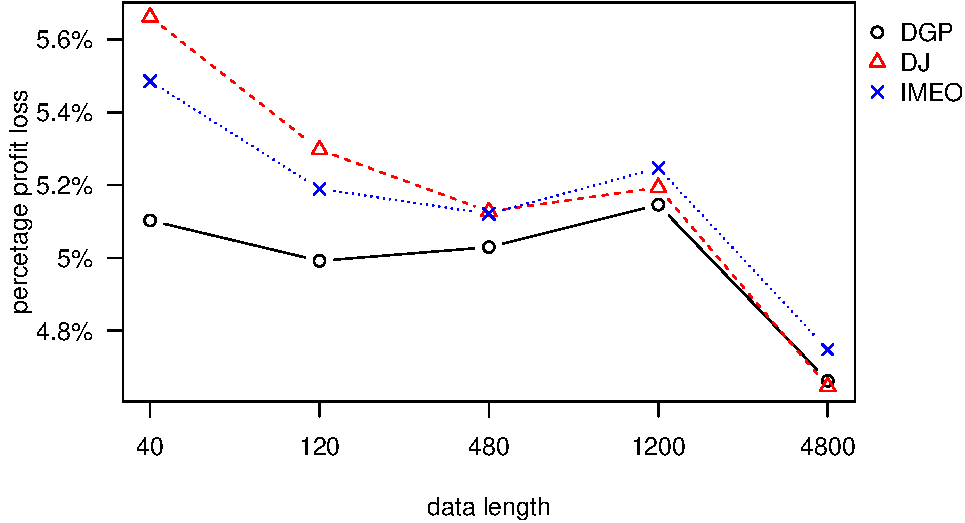
\includegraphics[width=\textwidth]{laplaceppl.pdf}
\caption{percentage profit loss vs. data size}
\end{subfigure}
\hfill
\begin{subfigure}[b]{0.48\textwidth}
\centering
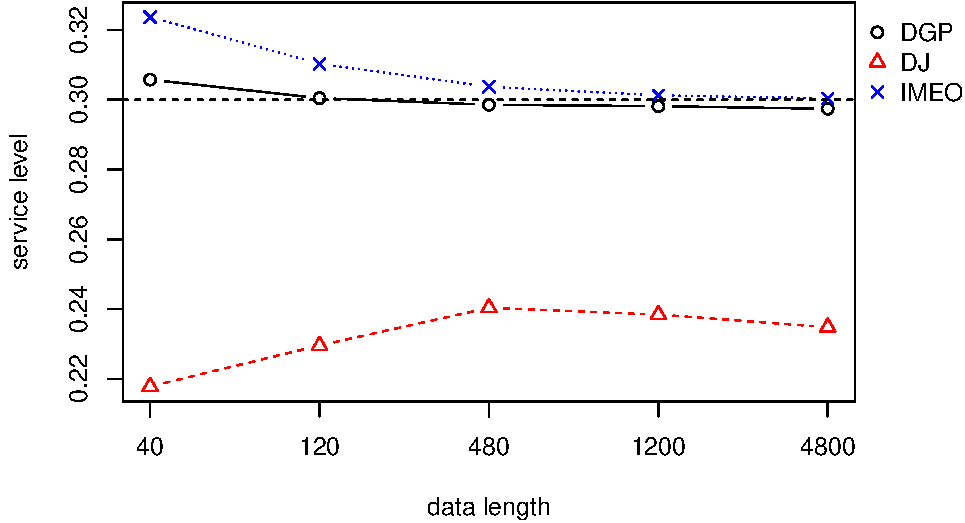
\includegraphics[width=\textwidth]{laplacesl.pdf}
\caption{service level vs. data size}
\end{subfigure}
\label{fig:err}
\end{figure}

As we see from this part of the experiment, IMEO is a robust approach, which works well in the case of misspecified model, even when the conventional disjoint method fails.


%%%%%%%%%% Wrong: Nonlinear case %%%%%%%%%%
\subsubsection{Nonlinear case} \label{sub:exp4}

Finally, we explore the case in which there is a nonlinear profit function and misspecification simultaneously. The same three scenarios of misspecification are considered.

\begin{figure}[ht]
\centering
\caption{Performance vs. sample size with under-parameterised nonlinear model}
\begin{subfigure}[b]{0.48\textwidth}
\centering
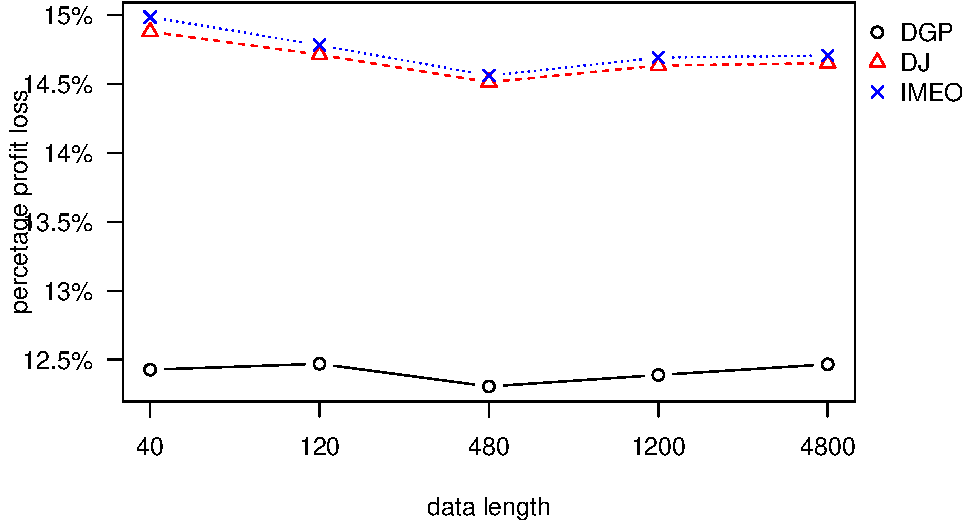
\includegraphics[width=\textwidth]{nonAR(1)ppl.pdf}
\caption{percentage profit loss vs. data size}
\end{subfigure}
\hfill
\begin{subfigure}[b]{0.48\textwidth}
\centering
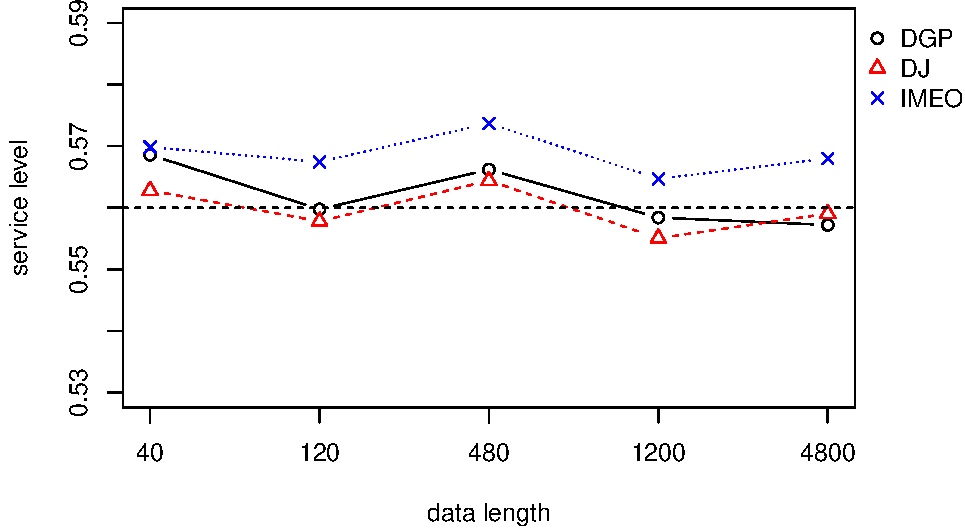
\includegraphics[width=\textwidth]{nonAR(1)sl.pdf}
\caption{service level vs. data size}
\end{subfigure}
\label{fig:misnon_under}
\end{figure}

Figure \ref{fig:misnon_under} represents the scenario in which the applied models are under-parameterised. We can see that the performance of methods in terms of PPL and SL are similar to the case of linear NVP discussed in Subsection \ref{sub:exp3}. The percentage profit loss for both DJ and IMEO stabilises around 14.75\% and never converges to the level of DGP due to the absence of the important variable in the model. This is compensated by SL, for which the DJ performs similar to DGP, with IMEO reaching slightly higher than needed level.

\begin{figure}[ht]
\centering
\caption{Performance vs. sample size with over-parameterised nonlinear model}
\begin{subfigure}[b]{0.48\textwidth}
\centering
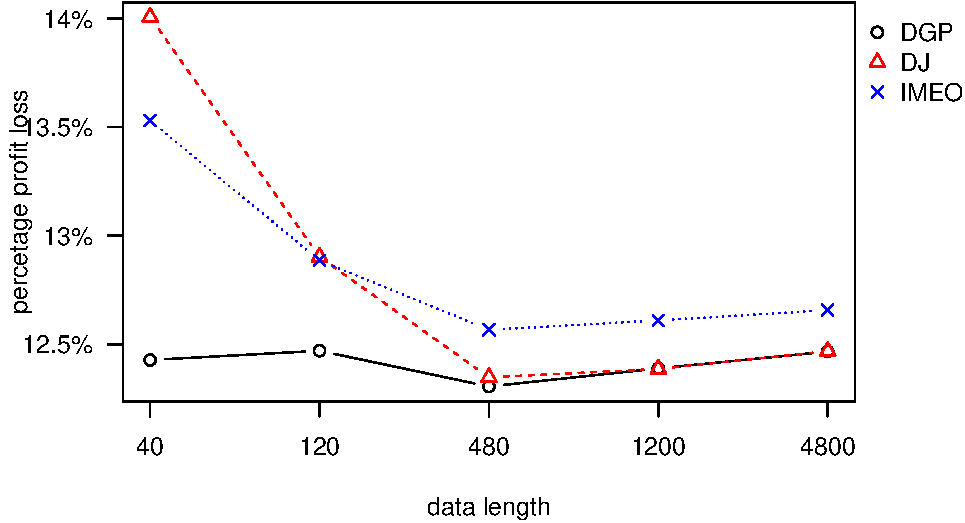
\includegraphics[width=\textwidth]{nonSAR(2)(1)_4ppl.pdf}
\caption{percentage profit loss vs. data size}
\end{subfigure}
\hfill
\begin{subfigure}[b]{0.48\textwidth}
\centering
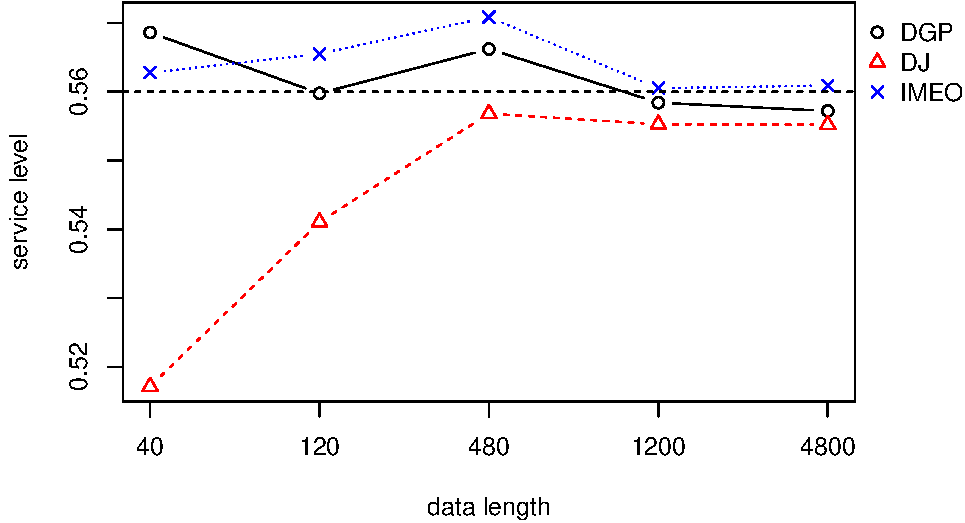
\includegraphics[width=\textwidth]{nonSAR(2)(1)_4sl.pdf}
\caption{service level vs. data size}
\end{subfigure}
\label{fig:misnon_over}
\end{figure}

Figure \ref{fig:misnon_over} demonstrates the over-parameterised scenario. We can see that IMEO has lower PPL than DJ on small samples, but with the increase of the sample size the latter method converges to the DGP, while IMEO still has a slight bias, producing around 0.1\% higher loss than the DGP. The good performance of IMEO on small samples could be because it does not require to estimate the variance of the error term. As for the SL, IMEO reaches the target level much faster than DJ, performing especially well on small samples, where the latter method reaches much lower service level than needed. As the smaple size increases, both methods converge to the target level.

Finally, we consider the scenario in which an incorrect distribution of error term is assumed. The results are presented in Figure \ref{fig:err_non}. It becomes apparent that IMEO outperform DJ in terms of PPL on small samples and converges to DGP together with DJ. It also performs more stable than DJ in terms of SL across all sample sizes. While it does not converge to the target level on larger samples, it is consistent and less biased than DJ, which converges to the value much higher than needed. One interesting thing we can see from both Figure \ref{fig:err_non} and Figure \ref{fig:err} is that the DJ always starts from a much lower than needed SL when sample size is small, and converges to a ``wrong", but higher, target as sample size grows. This ``wrong" target is obtained in both situation, not surprisingly, because DJ cannot overcome the incorrectness on distributional assumption.

Summarising this subsection, we see that IMEO is robust and does not fail as badly as the classical disjoint method does in sever cases of misspecification. At worst, IMEO performs similar to DJ.

\begin{figure}[ht]
\centering
\caption{Performance vs. sample size with Laplace distributed error term, nonlinear model}
\begin{subfigure}[b]{0.48\textwidth}
\centering
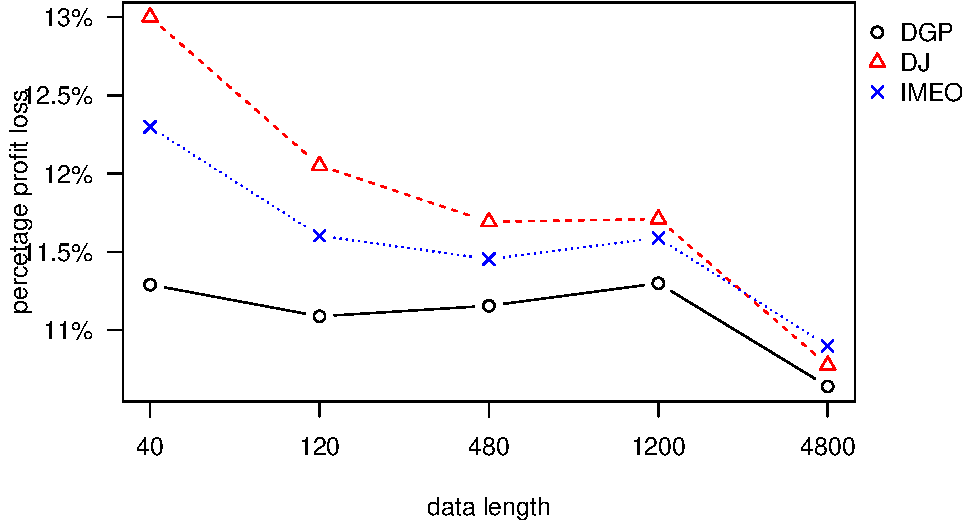
\includegraphics[width=\textwidth]{nonlaplaceppl.pdf}
\caption{percentage profit loss vs. data size}
\end{subfigure}
\hfill
\begin{subfigure}[b]{0.48\textwidth}
\centering
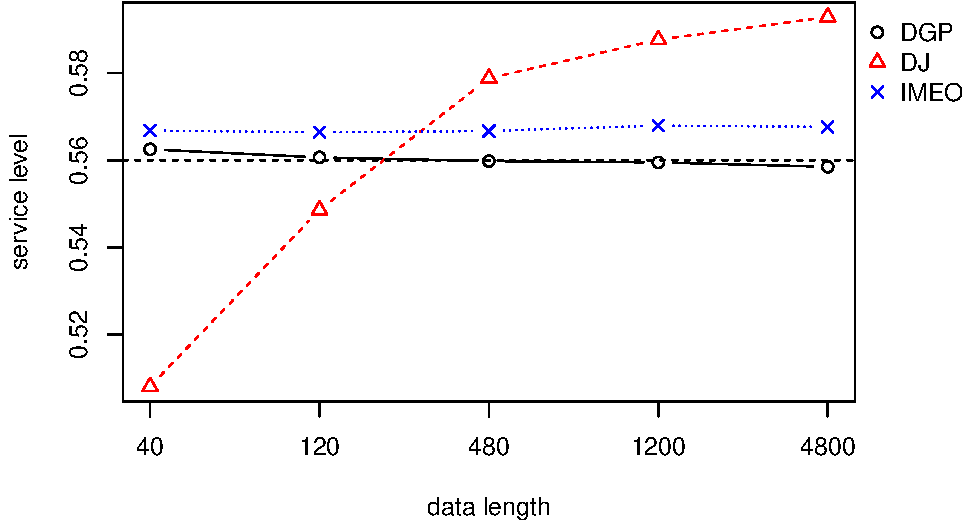
\includegraphics[width=\textwidth]{nonlaplacesl.pdf}
\caption{service level vs. data size}
\end{subfigure}
\label{fig:err_non}
\end{figure}


%%%%%%%%%% Conclusions %%%%%%%%%%
\section{Concluding Remarks} \label{se:end}

Newsvendor problem is one of the basic problems in stochastic programming. It is applicable to wide variety of real life situations, including, for example, dealing with perishable products and resources allocation. There are several methods for solving this problem, but they are either done sequentially in two steps (forecasting and optimisation) or rely on some assumptions about the problem at hands.

In this paper, we proposed a new approach called Integrated Method for Estimation and Optimisation (IMEO), due to which the estimation of a chosen model can be done using maximisation of the profit function directly instead of minimising a forecast error loss. We showed analytically that IMEO is equivalent to quantile regression in the simple (linear) case of NVP. This implies that the estimation of the optimal order quantity using IMEO is consistent, efficient and asymptotically normal for the linear NVP.

We then compared the performance of IMEO with conventional disjoint method and quantile regression in several simulation experiments, considering the situations in which the demand forecasting model is correctly specified and in which it is not. We showed that, when the true model is known, the proposed method performs similar to the quantile regression and to the disjoint method in classic NVP in terms of the percentage profit loss, service level and fill rate. When considering the situation with misspecified model, IMEO performs generally robustly, outperforming the disjoint method in some cases of model misspecification in terms of service level, and performs similarly in terms of other error measures. This becomes especially apparent, when the assumed distribution of error term is wrong.

Furthermore, we have tested the methods in the case of nonlinear NVP, and found that the proposed method performs at least as good as the disjoint one both in terms of percentage profit loss and service level, when the true model is known. However, when the applied model is wrong, IMEO does at least as good as the disjoint method in terms of percentage profit loss and much better in terms of achieved the service level.

All the conducted experiments demonstrate that the proposed method is robust and performs at least as good as the conventional ones in wide variety of cases, starting from utopic ones (when the true model is known) and ending with realistic ones, when some aspects of model are not known. Specifically, it does not fail as badly as the disjoint method in cases of sever model misspecification.

While the focus of this paper was on a specific ARIMA model, we expect that the obtained results could be generalised to other models as well, including regression and ETS, or even more complex nonlinear fitting methods, such as Machine Learning. Trying IMEO on these models and methods could be considered as a next step in our research.

While we have not studied the case of non-stationary data, we argue that the results of this paper are widely applicable to this case as well, because the scenarios under consideration inevitably come to the discussed in this paper: correct / misspecified model, linear / nonlinear NVP. Still more experiments on different types of models and model families can be considered as the future research as well.

Another interesting area of research is developing variables selection mechanism in IMEO: the conventional disjoint method allows doing this in the first stage either using cross-validation, or stepwise technique, but the proposed method does not have similar mechanism yet.

Finally, another potential direction of future research is multi-product NVPs, either with or without substitution effects between the products. The multivariate statistical models (such as vector autoregression and vector exponential smoothing) would be more suitable in this case, but it is not yet clear, whether any modifications would need to be done to the IMEO.

%%%%%%%%%%%%%%%%%%%%%%%%%%%%%%
% \newpage
% \begin{center}
% {\bf\Large Appendices}
% \end{center}

\appendix

\section{Proof of Scale and Shift Invariance}
\label{app:A}

\begin{proof}
For invariance with respect to scaling:
\[
    \begin{aligned}
        \hat{\boldsymbol{\beta}}(a\mathbf{y},\mathbf{X})
        &=\text{argmax}_{\boldsymbol{\beta}\in \mathbb{R}^{p+1}}\displaystyle\sum_{t=1}^s{\pi(\mathbf{x}_t^{\mathsf{T}}\boldsymbol{\beta},ay_t)}\\
        &=\text{argmin}_{\boldsymbol{\beta}\in \mathbb{R}^{p+1}}\displaystyle\sum_{t=1}^s{\{c_o[\mathbf{x}_t^{\mathsf{T}}\boldsymbol{\beta}-ay_t]^{+}+c_u[ay_t-\mathbf{x}_t^{\mathsf{T}}\boldsymbol{\beta}]^{+}\}}\\
        &=\text{argmax}_{\boldsymbol{\beta}\in \mathbb{R}^{p+1}}\displaystyle\sum_{t=1}^s{\pi\left(\mathbf{x}_t^{\mathsf{T}}\frac{\boldsymbol{\beta}}{a},y_t\right)}\\
        &=a\hat{\boldsymbol{\beta}}(\mathbf{y},\mathbf{X}).
    \end{aligned}
\]

\noindent
For invariance with respect to shifting:
\[
    \begin{aligned}
        \hat{\boldsymbol{\beta}}(\mathbf{y}+\mathbf{X}\gamma,\mathbf{X})
        &=\text{argmax}_{\boldsymbol{\beta}\in \mathbb{R}^{p+1}}\displaystyle\sum_{t=1}^s{\pi(\mathbf{x}_t^{\mathsf{T}}\boldsymbol{\beta},y_t+\mathbf{x}_t^{\mathsf{T}}\gamma)}\\
        &=\text{argmin}_{\boldsymbol{\beta}\in \mathbb{R}^{p+1}}\displaystyle\sum_{t=1}^s{\{c_o[\mathbf{x}_t^{\mathsf{T}}\boldsymbol{\beta}-y_t-\mathbf{x}_t^{\mathsf{T}}\gamma]^{+}+c_u[y_t+\mathbf{x}_t^{\mathsf{T}}\gamma-\mathbf{x}_t^{\mathsf{T}}\boldsymbol{\beta}]^{+}\}}\\
        &=\text{argmax}_{\boldsymbol{\beta}\in \mathbb{R}^{p+1}}\displaystyle\sum_{t=1}^s{\pi[\mathbf{x}_t^{\mathsf{T}}(\boldsymbol{\beta}-\gamma),y_t]}\\
        &=\hat{\boldsymbol{\beta}}(\mathbf{y},\mathbf{X})+\gamma.
    \end{aligned}
\]
\end{proof}

\section{Invariance under Reparameterization}
\label{app:B}
\begin{proof}
Define
    \[
        \mathbf{D}=\mathbf{X}A
        =\begin{pmatrix}
            \mathbf{d}_1^{\mathsf{T}}\\
            \mathbf{d}_2^{\mathsf{T}}\\
            \vdots\\
            \mathbf{d}_s^{\mathsf{T}}
        \end{pmatrix}
        =\begin{pmatrix}
            \mathbf{x}_{1}^{\mathsf{T}}\mathbf{a}^1&\mathbf{x}_1^{\mathsf{T}}\mathbf{a}^2&\cdots &\mathbf{x}_1^{\mathsf{T}}\mathbf{a}^{p+1}\\
            \mathbf{x}_2^{\mathsf{T}}\mathbf{a}^1&\mathbf{x}_2^{\mathsf{T}}\mathbf{a}^2&\cdots &\mathbf{x}_2^{\mathsf{T}}\mathbf{a}^{p+1}\\
            \vdots &\vdots &\ddots &\vdots \\
            \mathbf{x}_s^{\mathsf{T}}\mathbf{a}^1&\mathbf{x}_s^{\mathsf{T}}\mathbf{a}^2&\cdots &\mathbf{x}_s^{\mathsf{T}}\mathbf{a}^{p+1}
        \end{pmatrix},
    \]
    where $\mathbf{a}^n$ is the $n$th column of matrix $A$. We have
    \[
        \begin{aligned}
            &\hat{\boldsymbol{\beta}}(\mathbf{y},\mathbf{X}A)\\
            &\quad=\text{argmax}_{\boldsymbol{\beta}\in \mathbb{R}^{p+1}}\displaystyle\sum_{t=1}^s{\pi(\mathbf{d}_t^{\mathsf{T}}\boldsymbol{\beta},y_t)}\\
            &\quad=\text{argmin}_{\boldsymbol{\beta}\in \mathbb{R}^{p+1}}\displaystyle\sum_{t=1}^s{\{c_o[\mathbf{d}_t^{\mathsf{T}}\boldsymbol{\beta}-y_t]^{+}+c_u[y_t-\mathbf{d}_t^{\mathsf{T}}\boldsymbol{\beta}]^{+}\}}.
        \end{aligned}
    \]
    Note that
    \[
        \begin{aligned}
            \mathbf{d}_t^{\mathsf{T}}\boldsymbol{\beta}
            &=\displaystyle\sum_{n=1}^{p+1}\mathbf{x}_t^{\mathsf{T}}\mathbf{a}^n\beta_n\\
            &=\displaystyle\sum_{n=1}^{p+1}\displaystyle\sum_{m=1}^{p+1}x_{tm}a_{mn}\beta_n\\
            &=\displaystyle\sum_{m=1}^{p+1}x_{tm}\mathbf{a}_m^{\mathsf{T}}\boldsymbol{\beta}\\
            &=\mathbf{x}_t^{\mathsf{T}}A\boldsymbol{\beta},
        \end{aligned}
    \]
    where $a_{mn}$ is the element at $m$th row and $n$th column of $A$.
    From this, we have:
    \[
        \begin{aligned}
            &\hat{\boldsymbol{\beta}}(\mathbf{y},\mathbf{X}A)\\
            &\quad=\text{argmin}_{\boldsymbol{\beta}\in \mathbb{R}^{p+1}}\displaystyle\sum_{t=1}^s{\left\{c_o\left[\mathbf{x}_t^{\mathsf{T}}A\boldsymbol{\beta}-y_t\right]^{+}+c_u\left[y_t-\mathbf{x}_t^{\mathsf{T}}A\boldsymbol{\beta}\right]^{+}\right\}}\\
            &\quad=\text{argmax}_{\boldsymbol{\beta}\in \mathbb{R}^{p+1}}\displaystyle\sum_{t=1}^s{\pi(\mathbf{x}_t^{\mathsf{T}}A\boldsymbol{\beta},y_t)}\\
            &\quad=A^{-1}\hat{\boldsymbol{\beta}}(\mathbf{y},\mathbf{X}).
        \end{aligned}
    \]
\end{proof}
\section{Proof of Equivalence to Quantile Regression}
\label{app:C}
\begin{proof}
Here, we show that the loss function used in the proposed method is transformable to the typical loss function of quantile regression. In quantile regression, the loss function is defined as \cite{KH01}:
\[
    \hat{\boldsymbol{\beta}}=\text{argmin}_{\boldsymbol{\beta}\in \mathbb{R}^{p+1}}\displaystyle\sum_{t=1}^s\rho_{\tau}(y_t-\mathbf{x}_t^{\mathsf{T}}\boldsymbol{\beta}),
\]
where $\displaystyle \rho_{\tau}(u)=u(\tau-\mathbb{I}_{(u<0)})$, and $\mathbb{I}$ is an indicator function. Thus, all we need to do is to prove that:
\[
    \text{max}\displaystyle\sum_{t=1}^s{\pi(\mathbf{x}_t^{\mathsf{T}}\boldsymbol{\beta},y_t)}=\text{min}\displaystyle\sum_{t=1}^s\rho_{\tau}(y_t-\mathbf{x}_t^{\mathsf{T}}\boldsymbol{\beta}).
\]
We have:
\[
    \min[a,b]=a-[a-b]^+,
\]
and
\[
    a-b=[a-b]^+-[b-a]^+.
\]
We can transform:
\[
    \begin{aligned}
        \pi(\mathbf{x}_t^{\mathsf{T}}\boldsymbol{\beta},y_t)
        &=p\min[\mathbf{x}_t^{\mathsf{T}}\boldsymbol{\beta},y_t]-v\mathbf{x}_t^{\mathsf{T}}\boldsymbol{\beta}-c_h[\mathbf{x}_t^{\mathsf{T}}\boldsymbol{\beta}-y_t]^+-c_s[y_t-\mathbf{x}_t^{\mathsf{T}}\boldsymbol{\beta}]^+\\
        &=p\{\mathbf{x}_t^{\mathsf{T}}\boldsymbol{\beta}-[\mathbf{x}_t^{\mathsf{T}}\boldsymbol{\beta}-y_t]^+\}-v\mathbf{x}_t^{\mathsf{T}}\boldsymbol{\beta}-c_h[\mathbf{x}_t^{\mathsf{T}}\boldsymbol{\beta}-y_t]^+-c_s[y_t-\mathbf{x}_t^{\mathsf{T}}\boldsymbol{\beta}]^+\\
        &=(p-v)\mathbf{x}_t^{\mathsf{T}}\boldsymbol{\beta}-(c_h+p)[\mathbf{x}_t^{\mathsf{T}}\boldsymbol{\beta}-y_t]^+-c_s[y_t-\mathbf{x}_t^{\mathsf{T}}\boldsymbol{\beta}]^+.
    \end{aligned}
\]
Therefore, we have (since $y_t$ is fixed):
\[
    \begin{aligned}
        &\text{max}\displaystyle\sum_{t=1}^s{\pi(\mathbf{x}_t^{\mathsf{T}}\boldsymbol{\beta},y_t)}\\
        &\quad=\text{max}\displaystyle\sum_{t=1}^s\{(p-v)\mathbf{x}_t^{\mathsf{T}}\boldsymbol{\beta}-(c_h+p)[\mathbf{x}_t^{\mathsf{T}}\boldsymbol{\beta}-y_t]^+-c_s[y_t-\mathbf{x}_t^{\mathsf{T}}\boldsymbol{\beta}]^+\}\\
        &\quad=\text{max}\displaystyle\sum_{t=1}^s\{(p-v)[\mathbf{x}_t^{\mathsf{T}}\boldsymbol{\beta}-y_t]-(c_h+p)[\mathbf{x}_t^{\mathsf{T}}\boldsymbol{\beta}-y_t]^+-c_s[y_t-\mathbf{x}_t^{\mathsf{T}}\boldsymbol{\beta}]^+\}\\
        &\quad=\text{max}\displaystyle\sum_{t=1}^s\{(p-v)[\mathbf{x}_t^{\mathsf{T}}\boldsymbol{\beta}-y_t]^+-(p-v)[y_t-\mathbf{x}_t^{\mathsf{T}}\boldsymbol{\beta}]^+\\
        &\qquad-(c_h+p)[\mathbf{x}_t^{\mathsf{T}}\boldsymbol{\beta}-y_t]^+-c_s[y_t-\mathbf{x}_t^{\mathsf{T}}\boldsymbol{\beta}]^+\}\\
        &\quad=\text{min}\displaystyle\sum_{t=1}^s\{(v+c_h)[\mathbf{x}_t^{\mathsf{T}}\boldsymbol{\beta}-y_t]^++(p-v+c_s)[y_t-\mathbf{x}_t^{\mathsf{T}}\boldsymbol{\beta}]^+\}\\
        &\quad=\text{min}\displaystyle\sum_{t=1}^s\{c_o[\mathbf{x}_t^{\mathsf{T}}\boldsymbol{\beta}-y_t]^++c_u[y_t-\mathbf{x}_t^{\mathsf{T}}\boldsymbol{\beta}]^+\}.
    \end{aligned}
\]
By setting $\tau=\nicefrac{c_u}{(c_o+c_u)}$, we have:
\[
    \text{max}\displaystyle\sum_{t=1}^s{\pi(\mathbf{x}_t^{\mathsf{T}}\boldsymbol{\beta},y_t)}=\text{min}\displaystyle\sum_{t=1}^s\{(1-\tau)[\mathbf{x}_t^{\mathsf{T}}\boldsymbol{\beta}-y_t]^++\tau[y_t-\mathbf{x}_t^{\mathsf{T}}\boldsymbol{\beta}]^+\}=\text{min}\displaystyle\sum_{t=1}^s\rho_{\tau}(y_t-\mathbf{x}_t^{\mathsf{T}}\boldsymbol{\beta}).
\]
\end{proof}


%%%%%%%%%%%%%%%%%%%%%%%%%%%%%%
\printbibliography

\end{document}